\chapter{Conclusão}

\begin{figure}[htb]
	\centering
	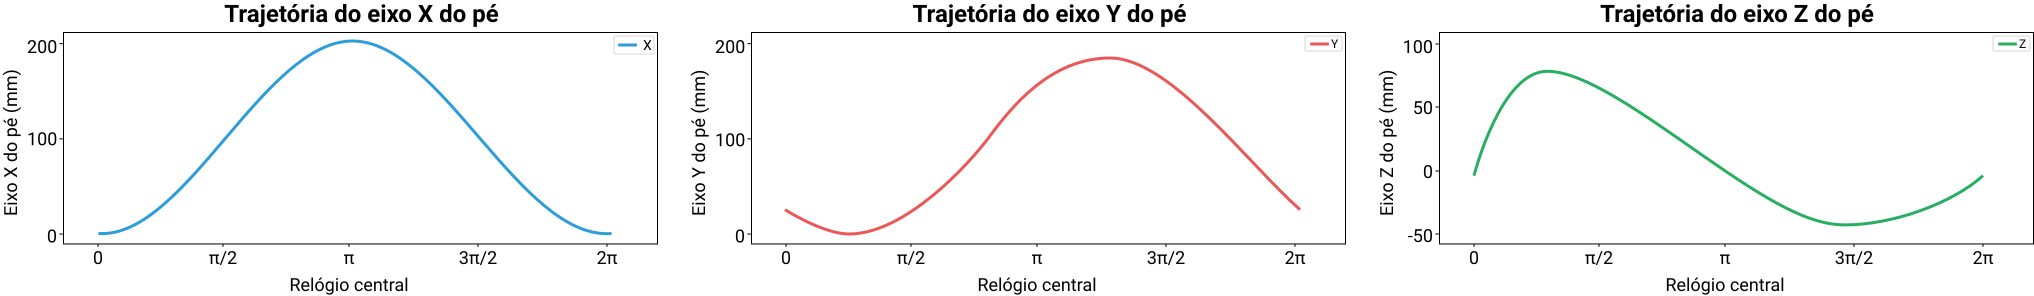
\includegraphics[width=\textwidth]{imagens/svg/conclusion-trajectories-graph}
	\caption{Gráficos do ciclo de caminhada nos eixos X, Y e Z.}
	\label{fig:conclusion:trajectories:graph}
\end{figure}

\begin{guide}
	Comparar com os resultados das trajetória mostrados por Kamiri.
\end{guide}

\begin{guide}
	Mostrar os frames da caminhada obtidos.
\end{guide}
	
As considerações finais formam a parte final (fechamento) do texto, sendo dito
de forma resumida (1) o que foi desenvolvido no presente trabalho e quais os
resultados do mesmo, (2) o que se pôde concluir após o desenvolvimento bem como
as principais contribuições do trabalho, e (3) perspectivas para o
desenvolvimento de trabalhos futuros, como listado nos exemplos de seção abaixo.
O texto referente às considerações finais do autor deve salientar a extensão e
os resultados da contribuição do trabalho e os argumentos utilizados estar
baseados em dados comprovados e fundamentados nos resultados e na discussão do
texto, contendo deduções lógicas correspondentes aos objetivos do trabalho,
propostos inicialmente.

\section{Trabalhos futuros}

As atualizações realizadas no \textit{walking gait} original do time AUTUofM agora permitem diversas expensões no código para futuras atualizações e investigações.

A implementação sem a utilização de um sistema de simulação apropriado não garante que o robô realmente possa caminhar. O uso do visualizador 3D apenas mostra um esboço do movimento, sem a real caminhada. Em paralelo, embora os dados do leitor de orientação sejam levados em conta tem todos os cálculos, seus efeitos não foram testados. Consequentemente, a integração do módulo do \textit{walking gait} a um \textit{framework} de simulação é um passo em direção a um sistema mais completo.

Segundo, durante uma tarefa genérica realizada por um robô não apenas se caminha. Movimentos como chutes, levantar-se do chão, pegar um copo -- entre outros -- são normalmente pré-gravados na etapa de desenvolvimento e durante a tarefa são apenas reproduzidos. Desta forma, um módulo para gravar e reproduzir estes movimentos faz-se necessário.

Terceiro, o fato do \textit{walking gait} rodar fora da \textit{OpenCM9.04} adiciona algum atraso extra entre o cálculo dos ângulos e a aplicação aos motores. Adicionalmente, os dados processados do leitor de orientação demoram mais a ter efeito nos cálculos das correções. Porém, o seu impacto real, durante a caminhada, não pode ser explorado neste trabalho deixando esta investigação para trabalhos futuros.

Quarto, alguns métodos de caminhada utilizam sensores nos pés de forma a detectar quando há o contato com o chão. Este momento é crítico pois, em caso de algum distúrbio, se houver uma diferença do momento esperado para o momento real do toque, ações diferenciadas poderão ser tomadas. Com isto em mente, sabe-se que os motores da série \textit{MX} possuem \textit{feedback} de carga baseado na voltagem de saída interna, onde deverá ser possível medir a diferença nas cargas esperadas e reais afim de prever se o pé está em contato com o chão.

Finalmente, outros métodos mais complexos de caminhada, utilizando mais processamento e mais memória, poderão ser implementados já que a barreira de recursos do \textit{OpenCM9.04} foi quebrada.